\documentclass[conference]{IEEEtran}
\usepackage{threeparttable}
\usepackage{color}
\usepackage{amsmath}
\usepackage{graphicx}
\usepackage{epstopdf}
%************ COMMENT BELOW WHEN NOT NEEDED ************%
%\usepackage{zref-totpages}
%\AtBeginDocument{
  %%\ifnum\ztotpages>6 %
    %\hypersetup{pdfstartpage=3,
		%%colorlinks = true, %Colors links instead of ugly boxes
		%%urlcolor = blue, %Color for external hyperlinks
		%%linkcolor = blue, %Color of internal links
		%%citecolor = red,  %Color of citations
		%}%
%%	\else
%%		\hypersetup{pdfstartpage=5}%
  %%\fi
%}
%\usepackage[pdftex,hidelinks]{hyperref}
%\usepackage{titlesec}
%\usepackage{indentfirst}
%************ END COMMENT ABOVE WHEN NOT NEEDED ************%
\newcommand{\rmnum}[1]{\romannumeral #1}
\newcommand{\Rmnum}[1]{\MakeUppercase{\romannumeral #1}}
\newcommand{\vect}[1]{\overline {#1}}
\newcommand{\vm}[1]{{\bf{#1}}}
\newcommand{\argmin}{\operatornamewithlimits{argmin}}
\newcommand{\argmax}{\operatornamewithlimits{argmax}}
\newcommand{\idxmin}{\operatornamewithlimits{idxmin}}
\newcommand{\idxmax}{\operatornamewithlimits{idxmax}}
\newcommand{\twopartdef}[4]
{
	\left\{
		\begin{array}{ll}
			#1 &; #2 \\
			#3 &; #4
		\end{array}
	\right.
}
\newcommand{\vecttwo}[2]
{
	\left[
		\begin{IEEEeqnarraybox*}[][c]{c}
		#1\\
		#2
		\end{IEEEeqnarraybox*}
	\right]
}
\newcommand{\vectthree}[3]
{
	\left[
		\begin{IEEEeqnarraybox*}[][c]{c}
		#1\\
		#2\\
		#3
		\end{IEEEeqnarraybox*}
	\right]
}
\begin{document}
\bstctlcite{IEEEexample:BSTcontrol}
% 
% paper title
% can use linebreaks \\ within to get better formatting as desired
\title{Color Shift Orthogonal Frequency Division Multiplexing}


% author names and affiliations
% use a multiple column layout for up to two different
% affiliations

\author{\IEEEauthorblockN{Pankil M. Butala, Hany Elgala, Thomas D.C. Little}
\IEEEauthorblockA{Department of Electrical and Computer Engineering\\
Boston University, Boston, MA, USA\\
\{pbutala, helgala, tdcl\}@bu.edu}
\and
\IEEEauthorblockN{Raed Mesleh}
\IEEEauthorblockA{Electrical Engineering Department\\
University of Tabuk, Tabuk, Saudi Arabia\\
rmesleh.sncs@ut.edu.sa}}

% make the title area
\maketitle

Visible light communications (VLC) are achieved by modulation of one or more spectral components in the visible spectrum ($\approx$400-800 nm). The use of this range provides an opportunity to exploit an otherwise untapped medium that is used in human lighting. Most visible light communication systems constructed to date focus on using a broad visible band generated by phosphor-converted blue light emitting diodes, or by filtering to isolate the blue components from these sources. Multi-wavelength systems consider multiple wavelength bands that are combined to produce the desired spectrum realizing a desired color temperature and intensity. The use of multiple bands is also a form of wavelength-division multiplexing. In this paper, we investigate the relationships between the colors comprising the lighting source for a range of lighting states, the spectral separation of communication channels, the relative intensities required to realize lighting states, how modulation can be most effectively mapped to the available color channels, and the design of an optical filtering approach to maximize SNR while minimizing crosstalk at the receiver. Simulation results based on a three colored VLC system are discussed using orthogonal frequency division multiplexing for each color. We show that the system is the most power efficient at 6250 K correlated color temperature, with transmitter spectral spread of 5 nm and filter transmittance width of 40 nm.

\begin{IEEEkeywords}
Visible Light Communications (VLC), Optical Wireless Communications (OWC), Multiple Input Multiple Output (MIMO), Color Shift Keying (CSK), Orthogonal Frequency Division Multiplexing (OFDM), IEEE 802.15.7
\end{IEEEkeywords}

\IEEEpeerreviewmaketitle
% introduction
\section{Introduction}
%Spectrum crunch. Solid state lighting wave. VLC as a means to mitigate downlink bottleneck.\\
%Smart spaces.  Multi-colored LEDs. Color tunability + WDM.\\
%ACO-OFDM. DCO-OFDM. O-OFDM background.\\
%In this work, find optimal range of operation for communication.
%O-OFDM over each color WDM + O-OFDM. More capacity.\\
There has been a rapid increase in use of networked portable computing devices in recent years. These devices are consuming increasingly more information in the form of multimedia streaming \cite{cis14a}. Trying to keep up with this increasing demand for wireless data has strained the network infrastructure thus creating the phenomenon of 'spectrum crunch'. Its effect can be seen in reduced quality of service and lower download speeds. 

On the other hand, advances made by the solid state industry has created energy efficient illumination devices called light emitting diodes (LED). The intensity of radiant flux emitted by LEDs can be modulated at a high enough rate such that information transfer can be achieved at relatively high speeds while the intensity variations are invisible to human eye. One or more LEDs can be packaged together to form a 'luminaire' which under the above model services the dual functionality of providing wireless network access and maintaining illumination \cite{kom04a}. The additional downlink capacity provided by such ``smart'' luminaires can help mitigate some of the aforementioned spectrum crunch.

A simple single input single output visible light communications (VLC) channel can be created by using an LED as a transmitter and a photodiode as a receiver. Channel characteristics for an optical channel are described in reference \cite{kah97a}. Another way of improving the capacity of a wireless channel is by using multiple transmitting and receiving elements in a multiple input multiple output (MIMO) configuration. Different types of MIMO systems \cite{hra06a,zen09a,ash10a,but13a,but14b} have been reported in literature.

One type of an optical MIMO system is wavelength division multiplexed (WDM) VLC system. Different WDM system prototypes have been reported in literature \cite{wan11a,kot12a,cos12a}. These describe an instance of a WDM system without analysis of the optimal operating point. In this work, design of multi-wavelength VLC systems under lighting constraints when correlated color temperature (CCT) of illumination, transmitter spectral power distribution (SPD) and receivers' filter spectral transmittance full width at half maximum (FWHM) are varied, is studied for the first time. Simulations for a three colored WDM VLC system then provide numerical analysis of the system performance giving an insight into optimal design criteria. For the system considered, we find that its most power efficient operation occurs at CCT of 6250 K, narrow transmitting elements' SPD (5 nm), and receiver filter FWHM of 40 nm.

The following notations are used in this paper. Scalar values are represented in regular font. Vectors and matrices are represented in bold font. Conjugate transpose of $\vm{A}$ is represented by $\vm{A}^{*}$. Operators $:=$ and $||.||$ represent definition and euclidean norm respectively. 

An introduction to optical MIMO systems is provided in Section \ref{sec:mimo}. WDM, a subset of optical MIMO systems, is introduced in Section \ref{sec:wdm}. Section \ref{sec:simulation} describes the simulation setup. Results and discussion is provided in Section \ref{sec:results}. Conclusions are then drawn in Section \ref{sec:conclusion}. 
% color shift keying
\section{Color Shift Keying}\label{sec:csk}

% cskofdm
\section{CS-OFDM}\label{sec:cskofdm}

% Simultion
\section{Simulation}\label{sec:simulation}
Simulations are performed to study how the choice of design parameters like illumination CCT, transmitter SPD, and filter FWHM affect the performance of a multi-wavelength VLC system. Three transmitting elements with Gaussian emission spectrum at dominant wavelengths of red (627 nm), green (530 nm) and blue (470 nm) are selected. Using these transmitting elements, CCT range of [2500 7000] K is sought. SPD spread within [5 50] nm is considered. \figurename{\ref{fig:LEDSPD}} illustrates normalized SPDs needed to achieve the range of CCTs for transmitting elements with 5 nm spread.

\begin{figure}[!b]
	\centering
		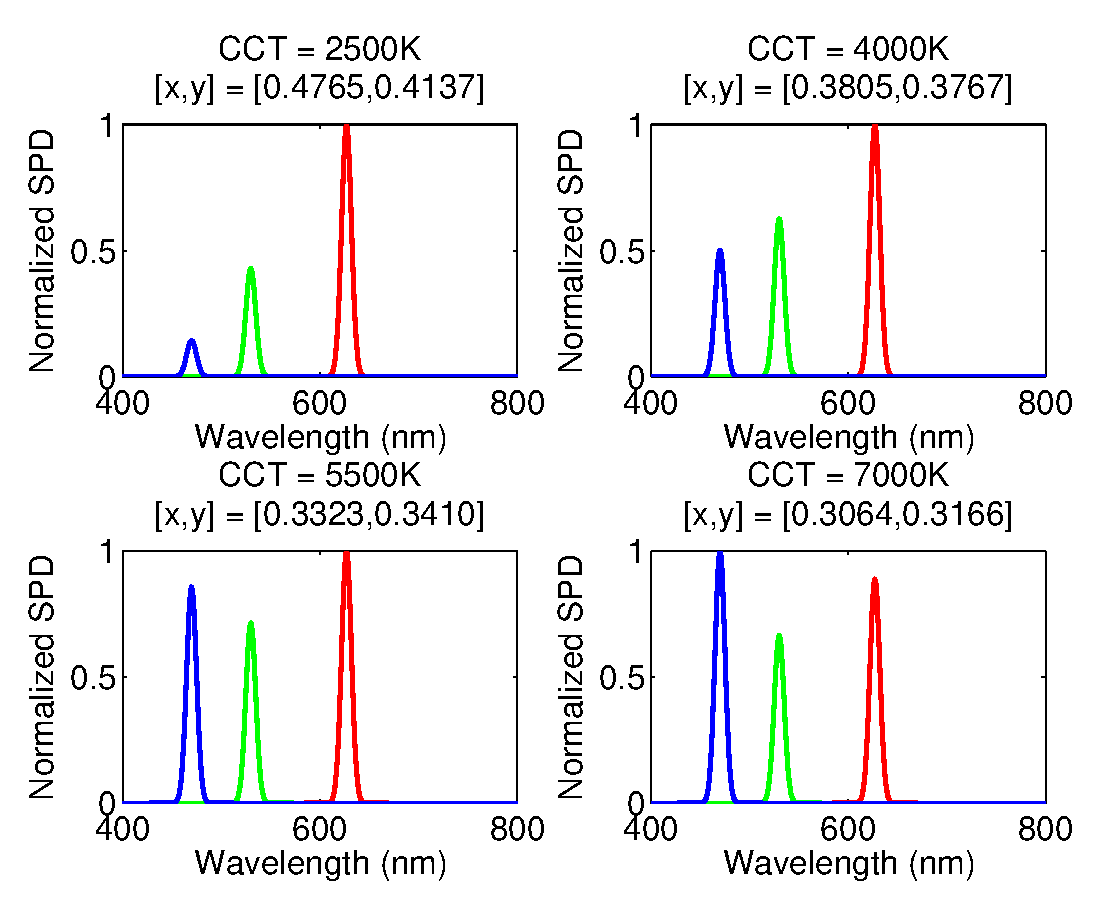
\includegraphics[trim={0.05in 0.05in 0.05in 0.0in}, clip=true, width=2.9in]{img/LEDSPD.eps}
	\caption{Transmitting element normalized spectral power distribution}
	\label{fig:LEDSPD}
\end{figure}

Unique $t_R:t_G:t_B$ ratios are generated after varying the tristimulus values in the range [0 1] in 0.1 unit steps. By substituting these values in Eq.(\ref{eqWhite})-Eq.(\ref{eqChromaticity}), chromaticity coordinates for resulting SPDs are calculated. An initial characterization step generates a pre-populated table consisting of the tristimulus values and corresponding chromaticity coordinates. As the CCT is varied, the chromaticity coordinates are computed as shown in Section \ref{sec:wdm}. From the pre-computed table, the tristimulus values that achieve the closest chromaticity are selected. The SPD is then scaled to achieve target illumination (400 lx) at the receiver that is located at a distance of 2 m from the transmitter. The surface normals of the transmitter and receiver are assumed to be parallel.

\begin{figure}[!t]
	\centering
		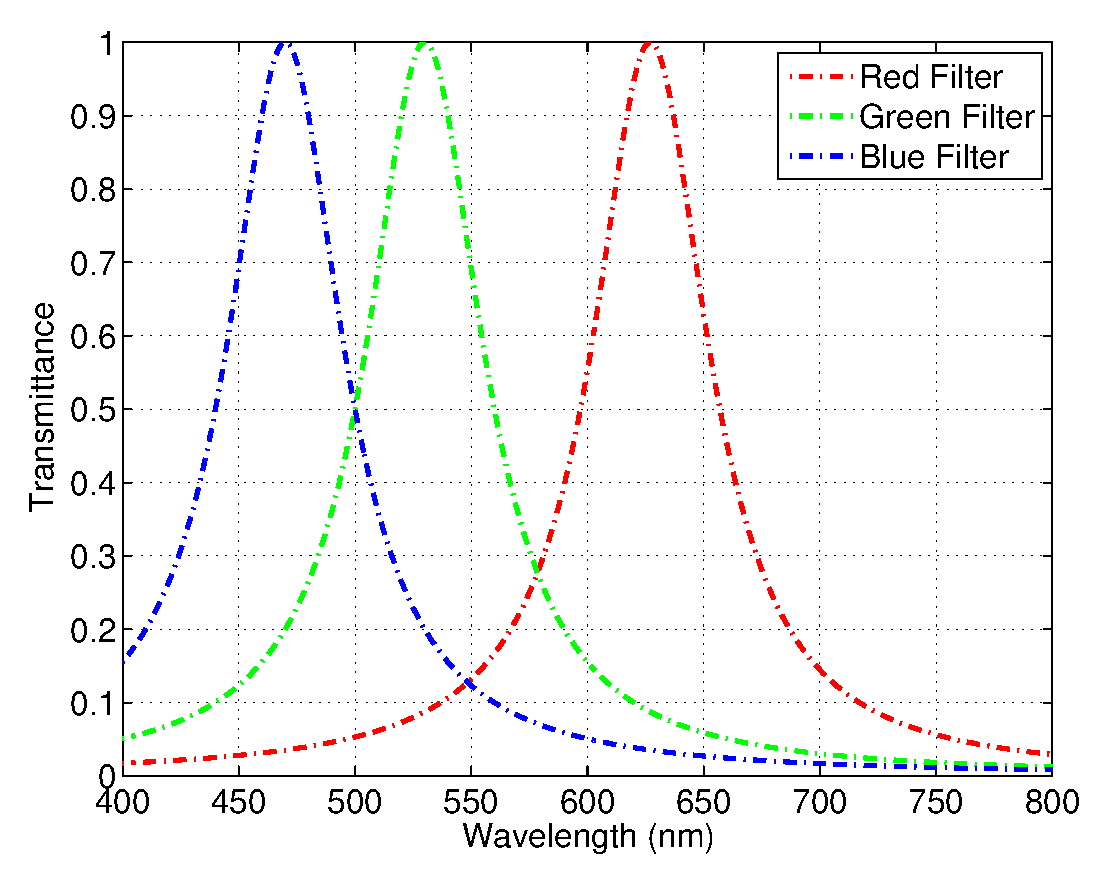
\includegraphics[trim={0.15in 0.05in 0.05in 0.35in}, clip=true, width=2.9in]{img/FiltTr.eps}
	\caption{Filter transmittance for full width at half maximum = 40nm}
	\label{fig:FiltTr}
\end{figure}

Optical filter's passband can be designed to center on the transmitting elements' dominant wavelengths. Optical filters for the simulation are modeled to have Lorentzian transmittance with ideal value $1$ at the dominant red, green and blue wavelengths mentioned above. Filter transmittance as a function of wavelength is illustrated in \figurename{\ref{fig:FiltTr}}. Filter FWHM considered for the analysis lie in [1 250] nm range.

The receiver sensor is assumed to be made of silicon. The assumed quantum efficiencies and responsivity of the sensor taken from source \cite{qeff} is illustrated in \figurename{\ref{fig:RecvResp}}. The responsivity near the blue wavelength is about 0.29 A.W$^{-1}$ and increases steadily to about 0.46 A.W$^{-1}$ near the red before rapidly reducing as the energy of the incident photon approaches the bandgap energy of silicon.

To analyze the system performance with reasonable number of iterations, transmitting and receiving elements are restricted to the same deviations about their respective means. A random bit stream is then generated. Bits for each link are then using asymmetrically clipped offset and DC-biased optical orthogonal frequency division multiplexing (ACO-OFDM and DCO-OFDM). Details on these optical OFDM techniques can be found in references \cite{car96a,arm06a}. For this simulation, ACO-OFDM and DCO-OFDM are implemented with 64 sub-carriers and 64-QAM and 8-QAM modulation, respectively. This ensures that both schemes achieve similar bits/symbol with ACO-OFDM achieving 96 bits/symbol and DCO-OFDM achieving 93 bits/symbol. The DC level on each link is set to ensure the desired CCT is achieved at the 400 lx illumination level. This generates the transmit vector $\vm{X}$. 

\begin{figure}[!b]
	\centering
		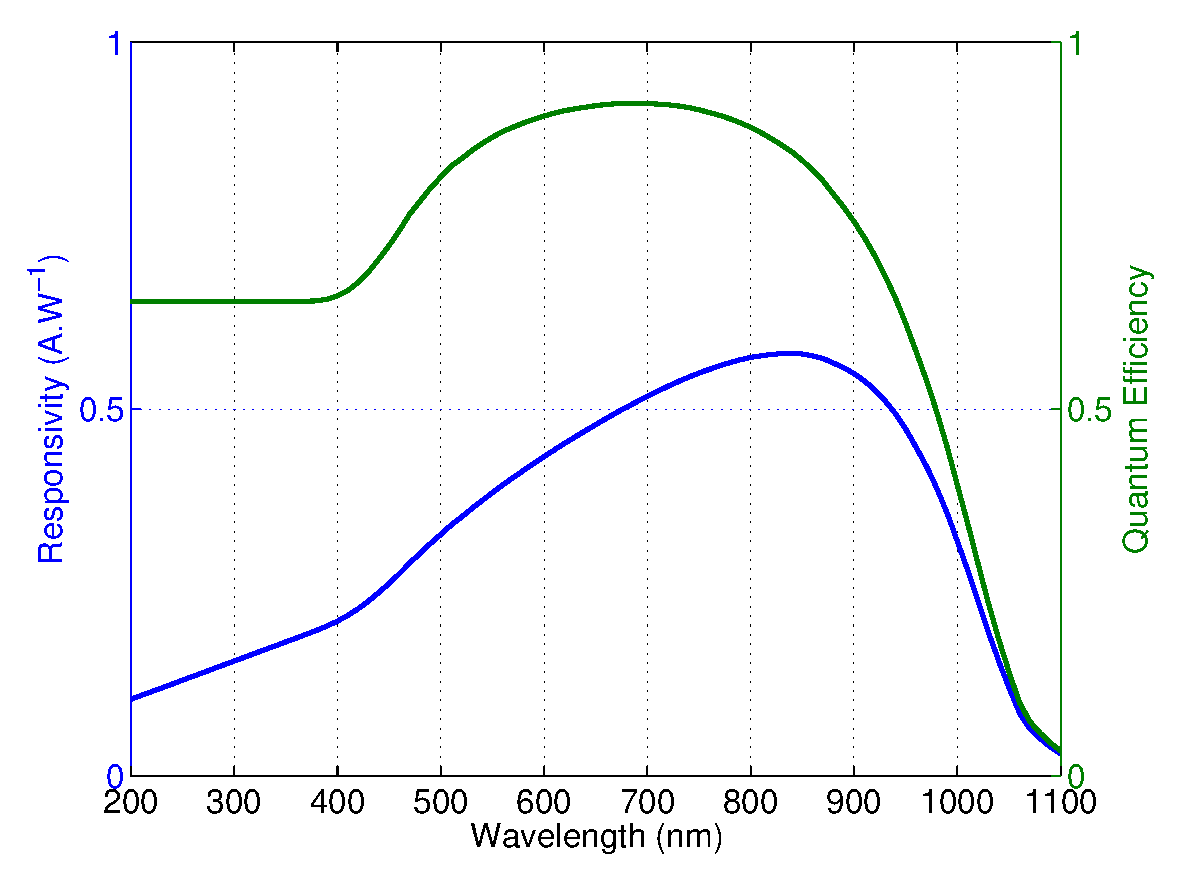
\includegraphics[trim={0.15in 0.05in 0.05in 0.0in}, clip=true, width=2.9in]{img/RecvResp.eps}
	\caption{Receiver quantum efficiency and responsivity \cite{qeff}}
	\label{fig:RecvResp}
\end{figure}

\begin{figure*}[tbph]
\centerline{\subfloat[Most power efficient operation point]{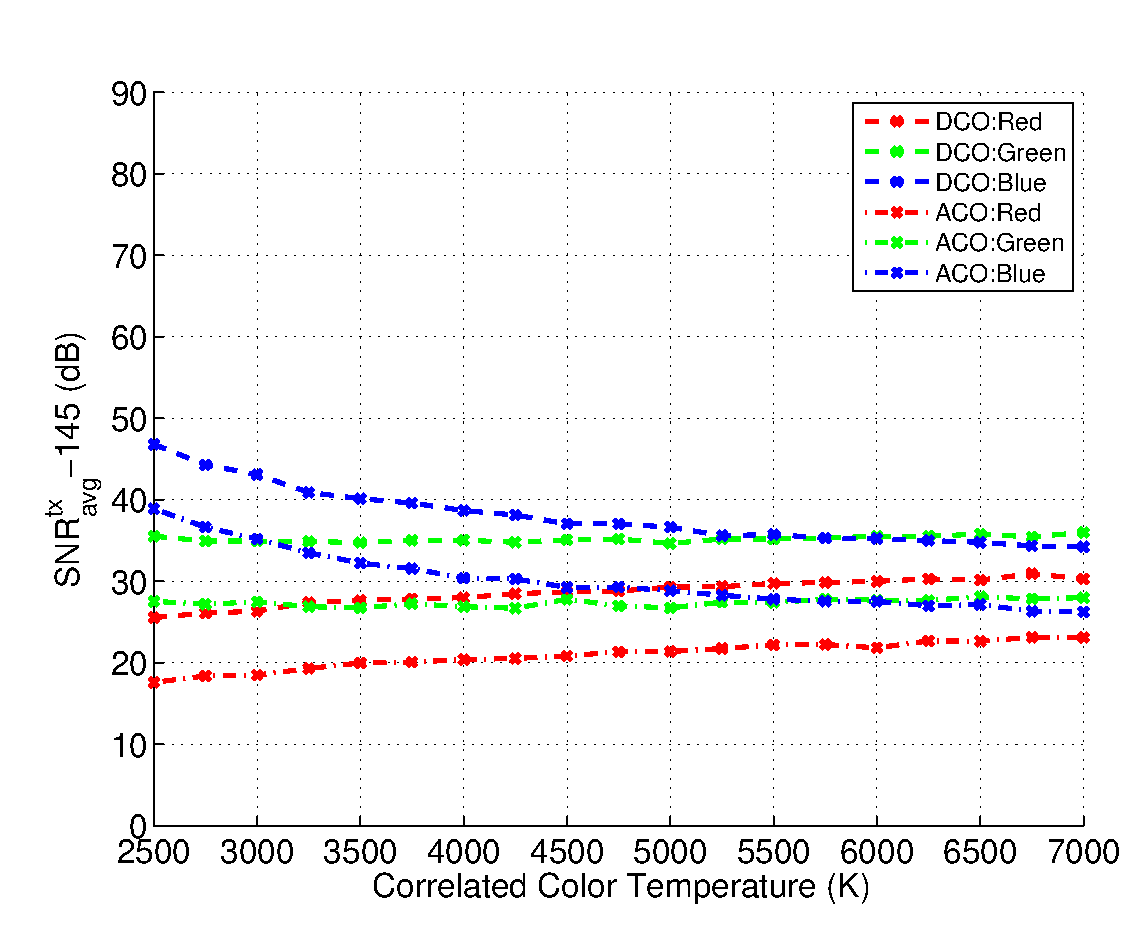
\includegraphics[trim={0.15in 0.05in 0.05in 0.35in}, clip=true, width=2.9in]{img/SNRvsCCT.eps} \label{subfig:SNRvsCCThigh}}
\hfil 
\subfloat[High inter-channel interference]{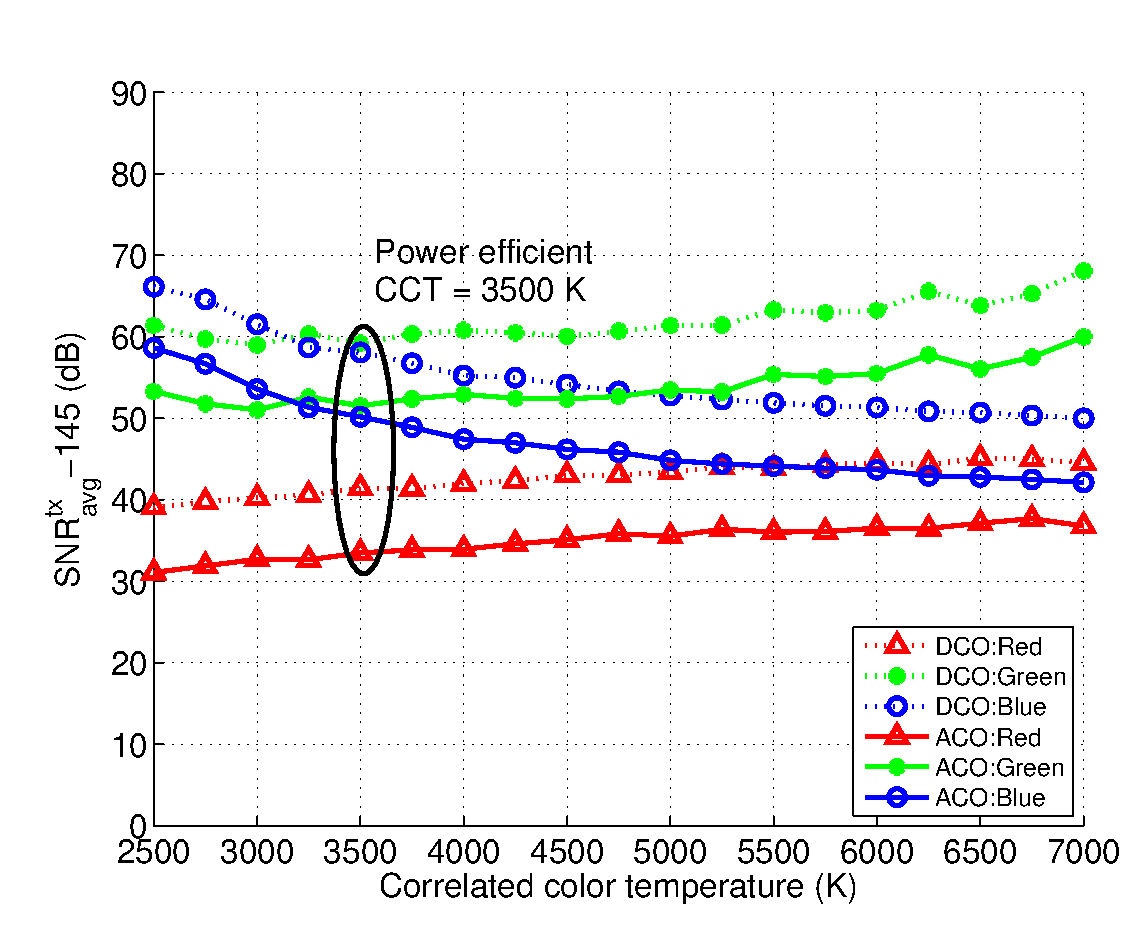
\includegraphics[trim={0.15in 0.05in 0.05in 0.35in}, clip=true, width=2.9in]{img/SNRvsCCT2.eps} \label{subfig:SNRvsCCTlow}}}
\caption{$\text{SNR}^{\text{tx}}_{\text{avg}}$ vs correlated color temperature to achieve BER $\leq 10^{-3}$ \newline(a) Transmitter: $\sigma_r = \sigma_g = \sigma_b = 5$ nm; Filter: $\Gamma_r = \Gamma_g = \Gamma_b = 40$ nm (b) Transmitter: $\sigma_r = \sigma_g = \sigma_b = 50$ nm; Filter: $\Gamma_r = \Gamma_g = \Gamma_b = 250$ nm}
\label{fig:SNRvsCCT}
\end{figure*}
\global\let\figone\relax

Having established $N_{tx} = 3$ transmitting and $N_{rx} = 3$ receiving elements, the $3\times 3$ channel matrix $\vm{H}$ can be computed as in Section \ref{sec:mimo}. AWGN vector $\vm{W}$ is generated and is then added to the transmitted vector. With the knowledge of the transmitted signal power and by varying the receiver noise, simulations over a range of $\text{SNR}^{\text{tx}}_{\text{avg}}$ are carried out. Vector \vm{Y} then collects the received signal and the added noise and interference. The least squares estimate of the transmitted signal vector is computed as
\begin{equation}
	\label{eqXhat}
	\hat{\vm{X}} = (\vm{H}^{*}\vm{H})^{-1}\vm{H}^{*}\vm{Y}
\end{equation}
An estimate of the transmitted optical OFDM frame for each color is obtained by aggregating least squares estimates of the received signal vectors. Further signal processing on each optical OFDM frame gets an estimate of the transmitted QAM symbol. Decoding the QAM symbols provides an estimate of the transmitted bits. Bit error rate (BER) is then calculated by comparing the transmit and estimated bit streams.


% Conclusion
\section{Conclusion}\label{sec:conclusion}
In this work, multi-wavelength VLC system in the context of variable illumination constraints was introduced. VLC system performance was characterized for variations in illumination CCT, transmitter SPD spread, and the receiver filter transmittance FWHM. For the three colored system considered, the blue and the green links pose the performance bottlenecks because of the relatively lower contribution to the SPD and lower photodiode responsivity as compared to the red. As the ICI increases, the most power efficient CCT shifts towards lower temperatures. Transmitting elements with the smallest spectral spread provide the most power efficient operating point. The effect of increase in spectral spread is most pronounced in the green link because it suffers the most from interference from the blue and red links. Filters with narrow transmittance FWHM reject a lot of the signal power while filters with a broad transmittance FWHM accept a lot of interference. Both of these affect the power efficiency of the system. For the setup considered, least power efficient operating point is for DCO-OFDM at CCT = 2500 K, transmitting element SPD spread = 50 nm, and filter FWHM = 1 nm. The most power efficient operating point is for ACO-OFDM at CCT = 6250 K, transmitting element SPD spread = 5 nm, and filter FWHM = 40 nm.
% Acknowledgement
\section{Acknowledgement}
This work was supported by the Engineering Research Centers Program of the National Science Foundation under NSF Cooperative Agreement No. EEC-0812056.
% Bibliography
\bibliographystyle{IEEEtran}
\bibliography{CSKOFDM}
\end{document}